\documentclass[
    12pt, % Schriftgröße
    DIV10,
    ngerman, % für Umlaute, Silbentrennung etc.
    a4paper, % Papierformat
    oneside, % einseitiges Dokument
    titlepage, % es wird eine Titelseite verwendet
    parskip=half, % Abstand zwischen Absätzen (halbe Zeile)
    headings=normal, % Größe der Überschriften verkleinern
    listof=totoc, % Verzeichnisse im Inhaltsverzeichnis aufführen
    bibliography=totoc, % Literaturverzeichnis im Inhaltsverzeichnis aufführen
    index=totoc, % Index im Inhaltsverzeichnis aufführen
    captions=tableheading, % Beschriftung von Tabellen unterhalb ausgeben
    final % Status des Dokuments (final/draft)
]{scrartcl}

% Pakete

% Schrift ----------------------------------------------------------------------
\usepackage{lmodern} % bessere Fonts

% Paket für Kopfzeilen und Fußzeilen
\usepackage[
    automark, % Kapitelangaben in Kopfzeile automatisch erstellen
    headsepline, % Trennlinie unter Kopfzeile
    ilines % Trennlinie linksbündig ausrichten
]{scrpage2}

% Anpassung an Landessprache
\usepackage[ngerman]{babel}

% Umlaute ----------------------------------------------------------------------
%   Umlaute/Sonderzeichen wie äöüß direkt im Quelltext verwenden (CodePage).
%   Erlaubt automatische Trennung von Worten mit Umlauten.
% ------------------------------------------------------------------------------
\usepackage[utf8]{inputenc}
\usepackage[T1]{fontenc}
\usepackage{textcomp} % Euro-Zeichen etc.

\usepackage[babel,german=quotes]{csquotes}

% Bei Änderungen müssen die *.aux und *.bbl Dateien manuell gelöscht werden
% Sonst kommt es zu einem Fehler bei der Erstellung
%\usepackage[round, sort, comma, numbers]{natbib}
%\usepackage[round, numbers]{natbib}
%\bibliographystyle{abbrvdin}
%

\usepackage{scrhack}

\usepackage[citestyle=alphabetic,bibstyle=alphabetic,backend=biber]{biblatex}
\bibliography{Bibliographie}
\DefineBibliographyStrings{german}{
  bibliography = {Literaturverzeichnis},
}
\setlength\bibitemsep{8pt}

\usepackage{xpatch}
\xpretobibmacro{author}{\mkbibbold\bgroup}{}{}
\xapptobibmacro{author}{\egroup}{}{}
\xpretobibmacro{editor}{\mkbibbold\bgroup}{}{}
\xapptobibmacro{editor}{\egroup}{}{}
\xpretobibmacro{editor+others}{\mkbibbold\bgroup}{}{}
\xapptobibmacro{editor+others}{\egroup}{}{}
\xpretobibmacro{bbx:editor}{\mkbibbold\bgroup}{}{}
\xapptobibmacro{bbx:editor}{\egroup}{}{}

% Grafiken ---------------------------------------------------------------------
% Einbinden von JPG-Grafiken ermöglichen
\usepackage[dvips,final]{graphicx}
\graphicspath{{Bilder/}}

% Paket zur Verwendung zusätzlicher Positionsbefehle
\usepackage{float}

% Befehle aus AMSTeX für mathematische Symbole z. B. \boldsymbol \mathbb --------
\usepackage{amsmath,amsfonts}

% Einfache Definition der Zeilenabstände und Seitenränder etc. -----------------
\usepackage{setspace}
\usepackage{geometry}

% zum Umfließen von Bildern ----------------------------------------------------
\usepackage{floatflt}

% Farbdefinitionen
\usepackage{xcolor} 
\definecolor{hellgelb}{rgb}{1,1,0.9}
\definecolor{colKeys}{rgb}{0,0,1}
\definecolor{colIdentifier}{rgb}{0,0,0}
\definecolor{colComments}{rgb}{1,0,0}
\definecolor{colString}{rgb}{0,0.5,0}
\definecolor{whgreen}{RGB}{113,177,41}
\definecolor{dvBlue}{RGB}{0,85,160}

% URL verlinken, lange URLs umbrechen etc. -------------------------------------
\usepackage{url}

% PDF-Optionen -----------------------------------------------------------------
\usepackage[
    bookmarks,
    bookmarksopen=true,
    colorlinks=true,
% diese Farbdefinitionen zeichnen Links im PDF farblich aus
    linkcolor=dvBlue, % einfache interne Verkn�pfungen
    anchorcolor=black,% Ankertext
    citecolor=dvBlue, % Verweise auf Literaturverzeichniseintr�ge im Text
    filecolor=magenta, % Verkn�pfungen, die lokale Dateien �ffnen
    menucolor=dvBlue, % Acrobat-Men�punkte
    urlcolor=dvBlue, 
% diese Farbdefinitionen sollten für den Druck verwendet werden (alles schwarz)
%    linkcolor=black, % einfache interne Verkn�pfungen
%    anchorcolor=black, % Ankertext
%    citecolor=black, % Verweise auf Literaturverzeichniseintr�ge im Text
%    filecolor=black, % Verkn�pfungen, die lokale Dateien �ffnen
%    menucolor=black, % Acrobat-Men�punkte
%    urlcolor=black, 
    %backref, % Inkompatibel mit BibLateX
    plainpages=false, % zur korrekten Erstellung der Bookmarks
    pdfpagelabels, % zur korrekten Erstellung der Bookmarks
    hypertexnames=false, % zur korrekten Erstellung der Bookmarks
    linktocpage % Seitenzahlen anstatt Text im Inhaltsverzeichnis verlinken
]{hyperref}

% fortlaufendes Durchnummerieren der Fußnoten ----------------------------------
\usepackage{chngcntr}
%\counterwithout{footnote}{chapter}

% Formatierung von Listen ändern -----------------------------------------------
\usepackage{paralist} % itemize, enumerate

% bei der Definition eigener Befehle benötigt
\usepackage{ifthen} % Vielleicht nicht nötig

% definiert u.a. die Befehle \ und \listoftodos
\usepackage{todonotes}
\reversemarginpar

% sorgt dafür, dass Leerzeichen hinter parameterlosen Makros nicht als Makroendezeichen interpretiert werden
\usepackage{xspace}

\usepackage{tabularx} % Tabellenspalten mit variabler Breite
\usepackage{wrapfig}  % Schriftumflossene Bilder


% Seitenstil

% Zeilenabstand 1,5 Zeilen
\onehalfspacing

% Seitenränder
% bottom is 20 + X, weil Footer nicht berücksichtigt wird
\geometry{paper=a4paper,left=30mm,right=20mm,top=20mm, bottom=38mm, footskip=8mm}

% Kopf- und Fußzeilen ----------------------------------------------------------
% Kopf- und Fußzeile auch auf Kapitelanfangsseiten
%\renewcommand*{\chapterpagestyle}{scrheadings} 
% Schriftform der Kopfzeile
%\renewcommand{\headfont}{\normalfont}

% Kopfzeile
\ihead{\headmark} % links
\chead{}
%\ohead{\includegraphics[scale=0.1]{Bilder/DJLogo.png}} % rechts
\setlength{\headheight}{20mm} % Höhe der Kopfzeile
% Kopfzeile über den Text hinaus verbreitern
%\setheadwidth[0pt]{textwithmarginpar} 
\setheadsepline[text]{0.4pt} % Trennlinie unter Kopfzeile

% Fußzeile
%\ifoot{} % links
\cfoot{} % mitte
\ofoot{\pagemark} % rechts
%\setfootsepline[text]{0.4pt} % Trennlinie unter Kopfzeile



% Schusterjungen und Hurenkinder vermeiden
%\clubpenalty = 10000
%\widowpenalty = 10000 
%\displaywidowpenalty = 10000

% Verringert den Abstand über den Überschriften
%\renewcommand*{\chapterheadstartvskip}{\vspace*{-\topskip}}

% Irgendwas mit Silbentrennung in MonoSpace (texttt)
\newcommand{\origttfamily}{}% sollte noch nicht definiert sein!
\let\origttfamily=\ttfamily % alte Definition von \ttfamily sichern
\renewcommand{\ttfamily}{\origttfamily \hyphenchar\font=`\-}


% Eigene Befehle und typographische Auszeichnungen für diese

\newcommand{\bs}{$\backslash$}

% einige Befehle zum Zitieren --------------------------------------------------
\newcommand{\Zitat}[2][\
empty]{\ifthenelse{\equal{#1}{\empty}}{\citep{#2}}{\citep[#1]{#2}}}

% zum Ausgeben von Autoren
\newcommand{\AutorName}[1]{\textsc{#1}}
\newcommand{\Autor}[1]{\AutorName{\citeauthor{#1}}}

% Produktnamen
\newcommand{\produkt}[1]{\textbf{#1}}

\newcommand{\code}[1]{\texttt{#1}}

% zum Einbinden von Programmcode -----------------------------------------------
\usepackage{listings}
\usepackage{xcolor}
\usepackage{textcomp}
\lstset{
    float=hbp,
    basicstyle=\ttfamily\color{black}\small,
    identifierstyle=\color{colIdentifier},
    keywordstyle=\color{colKeys},
    stringstyle=\color{colString},
    commentstyle=\color{colComments},
    %columns=flexible,
    tabsize=2,
    frame=single,
    extendedchars=true,
    showspaces=false,
    showstringspaces=false,
    numbers=left,
    numberstyle=\ttfamily\small,
    numbersep=5pt,
    breaklines=true,
    backgroundcolor=\color{hellgelb},
    breakautoindent=true
}

\lstset{literate=
  {á}{{\'a}}1 {é}{{\'e}}1 {í}{{\'i}}1 {ó}{{\'o}}1 {ú}{{\'u}}1
  {Á}{{\'A}}1 {É}{{\'E}}1 {Í}{{\'I}}1 {Ó}{{\'O}}1 {Ú}{{\'U}}1
  {à}{{\`a}}1 {è}{{\'e}}1 {ì}{{\`i}}1 {ò}{{\`o}}1 {ù}{{\`u}}1
  {À}{{\`A}}1 {È}{{\'E}}1 {Ì}{{\`I}}1 {Ò}{{\`O}}1 {Ù}{{\`U}}1
  {ä}{{\"a}}1 {ë}{{\"e}}1 {ï}{{\"i}}1 {ö}{{\"o}}1 {ü}{{\"u}}1
  {Ä}{{\"A}}1 {Ë}{{\"E}}1 {Ï}{{\"I}}1 {Ö}{{\"O}}1 {Ü}{{\"U}}1
  {â}{{\^a}}1 {ê}{{\^e}}1 {î}{{\^i}}1 {ô}{{\^o}}1 {û}{{\^u}}1
  {Â}{{\^A}}1 {Ê}{{\^E}}1 {Î}{{\^I}}1 {Ô}{{\^O}}1 {Û}{{\^U}}1
  {œ}{{\oe}}1 {Œ}{{\OE}}1 {æ}{{\ae}}1 {Æ}{{\AE}}1 {ß}{{\ss}}1 {Δ}{{$\Delta$}}1
  {ç}{{\c c}}1 {Ç}{{\c C}}1 {ø}{{\o}}1 {å}{{\r a}}1 {Å}{{\r A}}1
  {€}{{\EUR}}1 {£}{{\pounds}}1
}

\usepackage{microtype}

\renewcommand*{\dictumwidth}{.41\textwidth}
\renewcommand*{\dictumrule}{}
\renewcommand*{\dictumauthorformat}[1]{--- #1}
\setkomafont{dictumauthor}{%
\scshape
}

\definecolor{bluekeywords}{rgb}{0,0,1}
\definecolor{greencomments}{rgb}{0,0.5,0}
\definecolor{redstrings}{rgb}{0.64,0.08,0.08}
\definecolor{xmlcomments}{rgb}{0.5,0.5,0.5}
\definecolor{types}{rgb}{0.17,0.57,0.68}

\lstdefinestyle{csharp}
{
    language=[Sharp]C,
    captionpos=b,
    %numbers=left, %Nummerierung
    %numberstyle=\tiny, % kleine Zeilennummern
    showspaces=false,
    showtabs=false,
    breaklines=true,
    showstringspaces=false,
    breakatwhitespace=true,
    escapeinside={(*@}{@*)},
    commentstyle=\color{greencomments},
    morekeywords={partial, var, value, get, set},
    keywordstyle=\color{bluekeywords},
    stringstyle=\color{redstrings},
    basicstyle=\ttfamily\small,
}

\lstdefinestyle{hive}
{
    language=SQL,
    captionpos=b,
    %numbers=left, %Nummerierung
    %numberstyle=\tiny, % kleine Zeilennummern
    showspaces=false,
    showtabs=false,
    breaklines=true,
    showstringspaces=false,
    breakatwhitespace=true,
    escapeinside={(*@}{@*)},
    commentstyle=\color{greencomments},
    morekeywords={bigint, double, decimal, char, string, row, format, lines, location, DELIMITED, FIELDS, TERMINATED, STORED, TEXTFILE,
    	OVERWRITE, DIRECTORY},
    keywordstyle=\color{bluekeywords},
    stringstyle=\color{redstrings},
    basicstyle=\ttfamily\small,
}

\lstdefinestyle{xml}
{
    language=XML,
    captionpos=b,
    %numbers=left, %Nummerierung
    %numberstyle=\tiny, % kleine Zeilennummern
    showspaces=false,
    showtabs=false,
    breaklines=true,
    showstringspaces=false,
    breakatwhitespace=true,
    escapeinside={(*@}{@*)},
    commentstyle=\color{greencomments},
    morekeywords={encoding},
    keywordstyle=\color{bluekeywords},
    stringstyle=\color{redstrings},
    basicstyle=\ttfamily\small,
}

\colorlet{punct}{red!60!black}
\definecolor{background}{HTML}{EEEEEE}
\definecolor{delim}{RGB}{20,105,176}
\colorlet{numb}{magenta!60!black}

\lstdefinelanguage{json}{
    basicstyle=\normalfont\ttfamily,
    numbers=left,
    numberstyle=\scriptsize,
    stepnumber=1,
    numbersep=8pt,
    showstringspaces=false,
    breaklines=true,
    frame=single,
    literate=
     *{0}{{{\color{numb}0}}}{1}
      {1}{{{\color{numb}1}}}{1}
      {2}{{{\color{numb}2}}}{1}
      {3}{{{\color{numb}3}}}{1}
      {4}{{{\color{numb}4}}}{1}
      {5}{{{\color{numb}5}}}{1}
      {6}{{{\color{numb}6}}}{1}
      {7}{{{\color{numb}7}}}{1}
      {8}{{{\color{numb}8}}}{1}
      {9}{{{\color{numb}9}}}{1}
      {:}{{{\color{punct}{:}}}}{1}
      {,}{{{\color{punct}{,}}}}{1}
      {\{}{{{\color{delim}{\{}}}}{1}
      {\}}{{{\color{delim}{\}}}}}{1}
      {[}{{{\color{delim}{[}}}}{1}
      {]}{{{\color{delim}{]}}}}{1},
}

%\usepackage{caption} 
%\captionsetup[table]{skip=100pt}
% Bindet die Literaturdaten ein!
\bibliography{Bibliographie}
\begin{document}

%Startstruktur
\setcounter{secnumdepth}{3}
\setcounter{tocdepth}{2}

\pagestyle{empty}
\thispagestyle{plain}
\begin{titlepage}

\begin{center}


\includegraphics[scale=0.7]{Deckblatt/WH_Logo.jpg}

\vspace{2cm}

\Huge{\textbf{Autovermietung (DSL)}}\\[1.5ex]
\Large{\textbf{Projektdokumentation}}
\rule{\textwidth}{0.4pt}\\[3.0ex]

\large{\textbf{im Masterstudiengang Verteilte Systeme}}\\[3.0ex]

\normalsize
\begin{tabular}{ll}\\
	vorgelegt von: 
	& \quad Daniel Hardes, Fabian Paus \\[1.2ex]
	& \quad \\[1.2ex]
	Modul:  & \quad Business Process Management (BPM) \\[1.2ex]
	Gutachter:  & \quad Prof. Dr. Jürgen Priemer \\[1.2ex]
	Abgabetermin:  & \quad 2. Februar 2016\\[1.2ex]
\end{tabular}

\end{center}

\end{titlepage}


\tableofcontents
\setcounter{page}{1}

\pagestyle{scrheadings}

\newpage

\section{Einleitung}

Aufgabe dieses Projekts war es eine Autovermietung mithilfe von jBPM und Drools zu erstellen. Die Geschäftsregeln sollen am Ende über eine Domain-Specific-Language (DSL) verwaltet werden. Zur Definition der Regeln wurden die dreizehn Aussagen aus der Aufgabenstellung analysiert und ausgewertet. 

Im Laufe dieser Projektdokumentation werden die einzelnen Arbeitsschritte strukturiert und detailliert beschrieben. Der Quellcode und die Projektdokumentation kann über ein öffentliches Git-Repository (\url{https://github.com/fabian-paus/car-rental}) auf GitHub.com eingesehen werden. 

Als Ergebnis haben wir eine grafische Benutzeroberfläche entworfen, über die eine Mietanfrage an die Prozess-Engine gesendet werden kann. Die Prozess-Engine verarbeitet die Anfrage und nutzt die Regel-Engine zur Ausführung von Geschäftsregeln.
Unter gewissen Bedingungen muss der Filialleiter einen Schritt genehmigen.
Am Ende wird die Anfrage entweder angenommen oder abgelehnt. Eine angenommene Anfrage enthält dann eine Fahrzeugklasse und einen Gesamtpreis. Diese Daten werden dann über die Oberfläche an den Benutzer ausgegeben. 

\section{Einarbeitung}

Um die Aufgabe besser zu strukturieren definieren wir zunächst einige Domänenbegriffe und 
beschreiben dann den Ablauf des Vermietungsprozesses mithilfe eines Flussdiagramms.

\subsection{Domänenbegriffe}

In diesem Abschnitt werden Begriffe, die für den Vermietungsprozess wichtig sind, definiert.
Diese Begriffe werden in Diagrammen, in Regeln und bei der Prozessdefinition verwendet.
Einige Begriffe werden nicht exakt definiert, da diese später in Regeln genauer
festgelegt werden.

\begin{description}
	\item[Kunde:] Ein Kunde möchte einen Wagen mieten. Für jeden Kunden sind folgende Eigenschaften bekannt:
		\begin{description}
			\item[Alter:] Wie alt ist der Kunde? Einheit: Jahre
			\item[Führerscheindauer:] Wie lange hat der Kunde seinen Führerschein? Einheit: Jahre
			\item[Sicherheitstraining:] Hat der Kunde ein Fahrsicherheitstraining absolviert?
			\item[Reklamation:] Hat der Kunde eine berechtigte Reklamation vorgebracht?
			\item[Neukunde:] Ist der Kunde zum ersten Mal bei der Autovermietung?
		\end{description}
	\item[Fahranfänger] Ein Kunde ist ein Fahranfänger, wenn er jünger als ein bestimmtes Alter ist oder
		seinen Führerschein noch nicht sehr lange besitzt. Die genaue Definition erfolgt anhand einer
		Geschäftsregel.	
	\item[Filialleiter:] Gewisse Entscheidung beim Vermietungsprozess bedürfen der Genehmigung durch
		den Filialleiter.
	\item[Klasse:] Ein zu mietender Wagen wird in vier Klassen eingeteilt:
		\begin{description}
			\item[Klein:] Kleinwagen
			\item[Kompakt:] Kompaktwagen
			\item[Mittel:] Mittelklassewagen
			\item[Ober] Oberklassewagen
		\end{description}
	\item[Anfrage:] Eine Anfrage für einen Mietwagen wird von einem Kunden gestellt. Sie enthält folgende Informationen:
		\begin{description}
			\item[Fahrer:] Welche Kunden fahren mit dem Auto? (Achtung: mehr als ein Fahrer möglich)
			\item[Startdatum:] Ab welchem Datum wird das Auto gemietet? Einheit: Datum
			\item[Dauer:] Für wie lange soll das Auto gemietet werden? Einheit: Tage
			\item[Klasse:] Welche Wagenklasse soll gemietet werden? Einheit: Klasse (siehe Definition oben)
			\item[Automatik:] Soll der Mietwagen eine Automatikschaltung haben?
		\end{description}
	\item[Tagespreis:] Der Tagespreis ist der Preis für eine Mietdauer von einem Tag. Einheit: Euro
	\item[Basispreis:] Der Basispreis ist die Summe der Tagespreise über die gesamte Dauer. Einheit: Euro
	\item[Rabatt:] Der Rabatt ist ein Nachlass, der auf Kundenbasis ermittelt wird. Einheit: Euro
	\item[Automatikgebühr:] Eine zusätzliche Gebühr, falls ein Automatikwagen gemietet wird. Einheit: Euro
	\item[Endpreis:] Der Endpreis wird aus dem Basispreis, dem Rabatt und der Automatikgebühr berechnet. Einheit: Euro
	\item[Zuschlag:] Ein prozentualer Zuschlag auf den Endpreis. Einheit: Prozent
	\item[Nachlass:] Ein prozentualer Nachlass auf den Endpreis. Einheit: Prozent
	\item[Gesamtpreis:] Nachdem Zuschlag und Nachlass auf den Endpreis berechnet wurden, ergibt sich der Gesamtpreis. Einheit: Euro
	
\end{description}

\subsection{Flussdiagramm}

Anhand des Flussdiagramms beschreiben wir den gesamten Vermietungsprozess. Dabei gehen wir auf
die einzelnen Aussagen aus der Aufgabenstellung ein.

\subsubsection{Gesamter Prozess}

Wir haben den gesamten Prozess in drei Teilprozesse unterteilt:
\begin{enumerate}
	\item Fahranfängerprüfung
	\item Verfügbarkeitsprüfung
	\item Preisberechnung
\end{enumerate}

Nach Aussage 3 wird zuerst geprüft, ob die Anfrage die maximale Dauer überschreitet.

\begin{figure}[tbh]
\centering
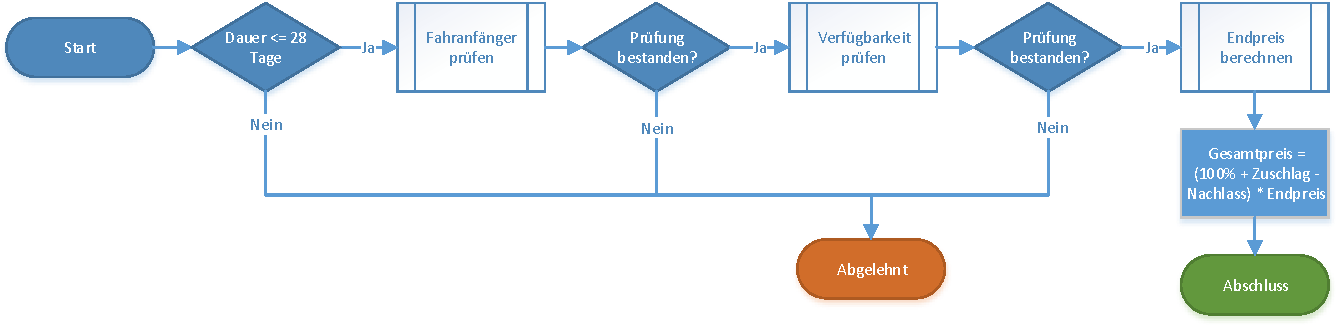
\includegraphics[width=1.0\linewidth]{Bilder/Preis_berechnen}
\caption{Preisfindung}
\label{fig:Preis_berechnen}
\end{figure}

\subsubsection{Fahranfängerprüfung}

In Aussage 10 wird definiert, wer als Fahranfänger eingestuft wird, und welcher Aufschlag in dem 
Fall zu zahlen ist. Aussage 11 bestimmt die Fahrzeugklassen, die nur mit Genehmigung vom Filialleiter
durch Fahranfängern gemietet werden dürfen.

\begin{figure}[H]
\centering
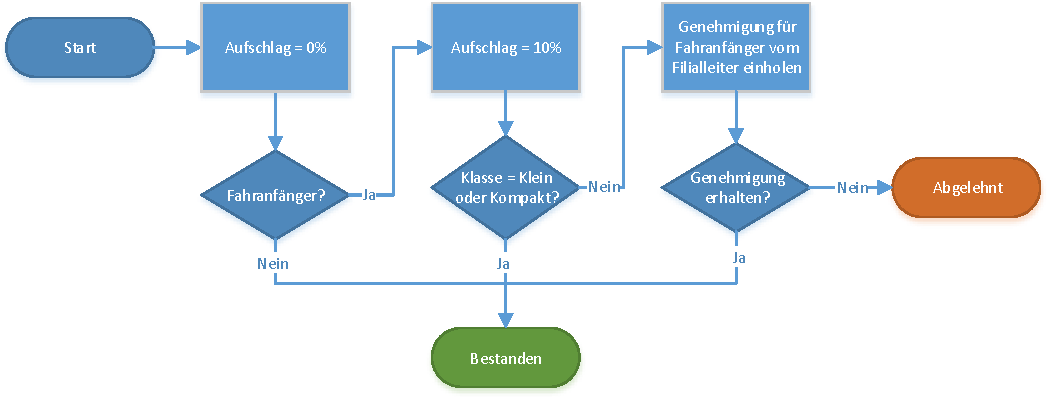
\includegraphics[width=0.8\linewidth]{Bilder/Fahranfaenger_pruefen}
\caption{Fahranfängerprüfung}
\label{fig:Fahranfänger_prüfen}
\end{figure}

\subsubsection{Verfügbarkeitsprüfung}

Aussagen: 12 (Kostenloses Upgrade nach Genehmigung), 13 (Downgrade aus Oberklasse)

In Aussage 12 wird beschrieben, was passieren soll, wenn kein Fahrzeug der angefragten Klasse
verfügbar ist. Dann wird nach Genehmigung durch den Filialleiter ein kostenloses Upgrade 
auf die nächsthöhere Klasse durchgeführt. 
Aussage 13 erläutert den Fall, wenn kein Oberklassewagen verfügbar ist. In dem Fall wird
ein Downgrade auf die Mittelklasse durchgeführt mit zusätzlichem Nachlass auf den Endpreis.

\begin{figure}[H]
\centering
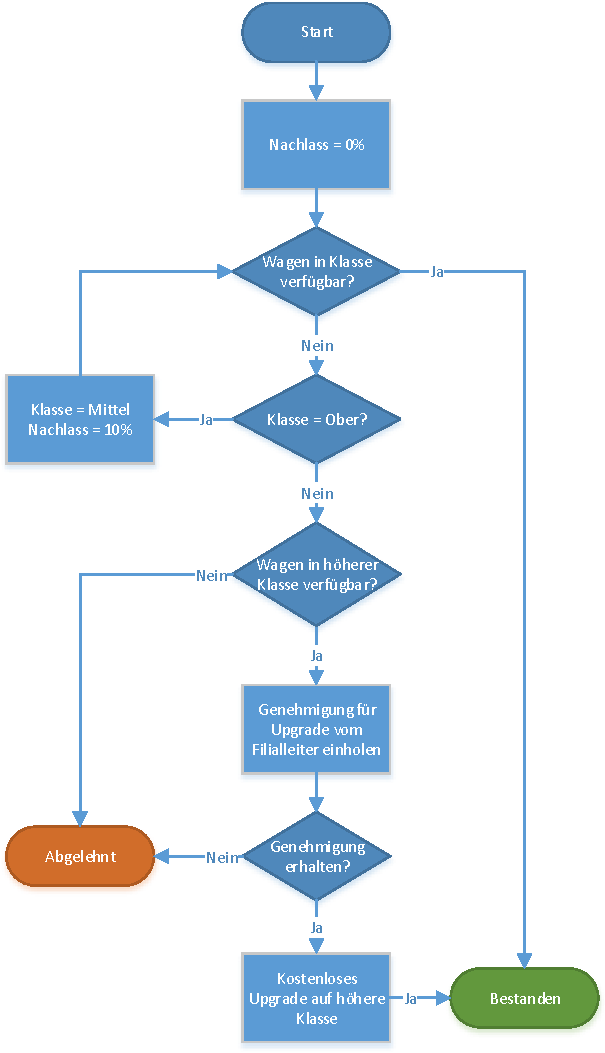
\includegraphics[width=0.55\linewidth]{Bilder/Verfuegbarkeit_pruefen}
\caption{Verfügbarkeitsprüfung}
\label{fig:Verfuegbarkeit_pruefen}
\end{figure}

\subsubsection{Preisberechnung}

Die Preisberechnung besteht aus drei Schritten:
\begin{enumerate}
	\item Basispreisberechnung
	\item Rabattberechnung
	\item Automatikgebühr (nach Aussage 8)
\end{enumerate}

Der Endpreis setzt sich aus dem Basispreis abzüglich des Rabatts und zuzüglich 
der Automatikgebühr zusammen.

\begin{figure}[H]
	\centering
	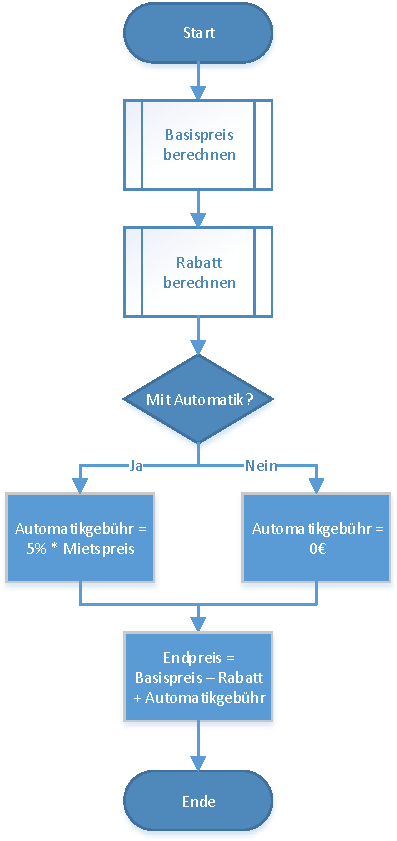
\includegraphics[width=0.4\linewidth]{Bilder/Endpreis_berechnen}
	\caption{Endpreis berechnen}
	\label{fig:Endpreis_berechnen}
\end{figure}

\newpage 
\paragraph{Basispreis}

Der Basispreis entspricht der Summe aller Tagespreise.

\begin{figure}[H]
	\centering
	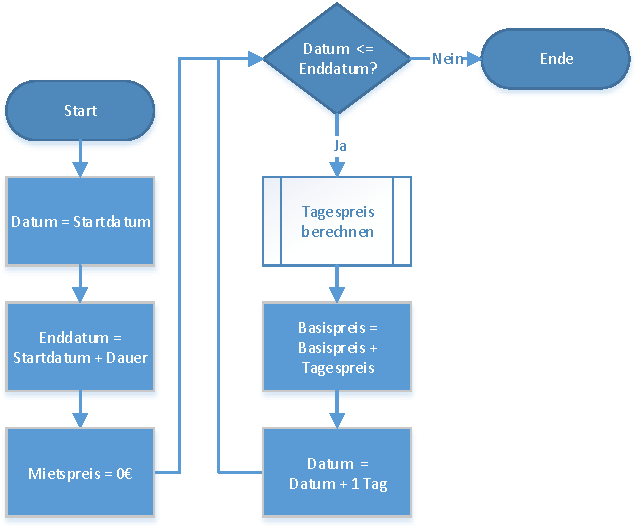
\includegraphics[width=1.0\linewidth]{Bilder/Basispreis_berechnen}
	\caption{Basispreis berechnen}
	\label{fig:Basispreis_berechnen}
\end{figure}

\paragraph{Tagespreis}

Bei der Tagespreisberechnung werden die Aussagen 1, 2 und 3 berücksichtigt.

Aussage 1 bestimmt den Tagespreis in Abhängigkeit von der Fahrzeugklasse.
Der Tagespreis wird allerdings an Wochenenden und Feiertagen nach Aussage 2
reduziert. Außerdem ist jeder siebte Tag nach Aussage 3 kostenlos.

\begin{figure}[H]
	\centering
	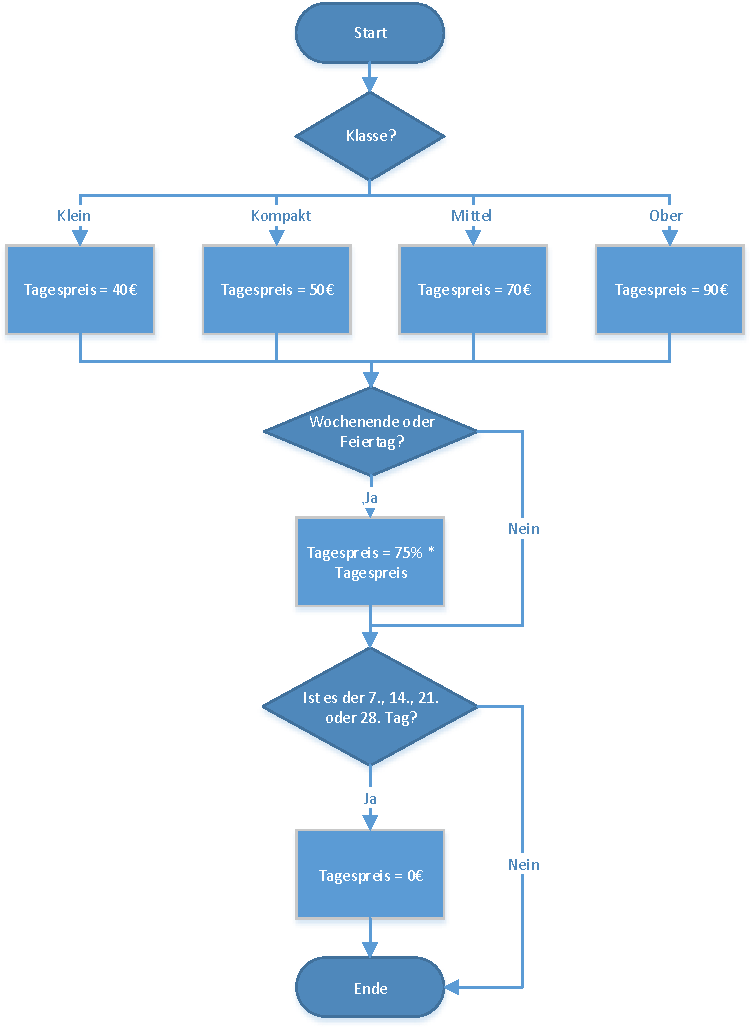
\includegraphics[width=0.9\linewidth]{Bilder/Tagespreis_berechnen}
	\caption{Tagespreis berechnen}
	\label{fig:Tagespreis_berechnen}
\end{figure}

\paragraph{Rabatt}

Bei der Rabattberechnung werden laut Aussagen 4, 5 und 6 die Eigenschaften Neukunde, alte Reklamation
und Sicherheitstraining berücksichtigt. Dabei ist zu beachten, dass bei mehreren Fahrern die
schlechteren Konditionen gelten. Das haben wir über die "`Alle Fahrer"'-Bedingungen abgebildet (Aussage 7). Außerdem darf nach Aussage 9 der Rabatt eine bestimmte Grenze nicht überschreiten.

\begin{figure}[H]
	\centering
	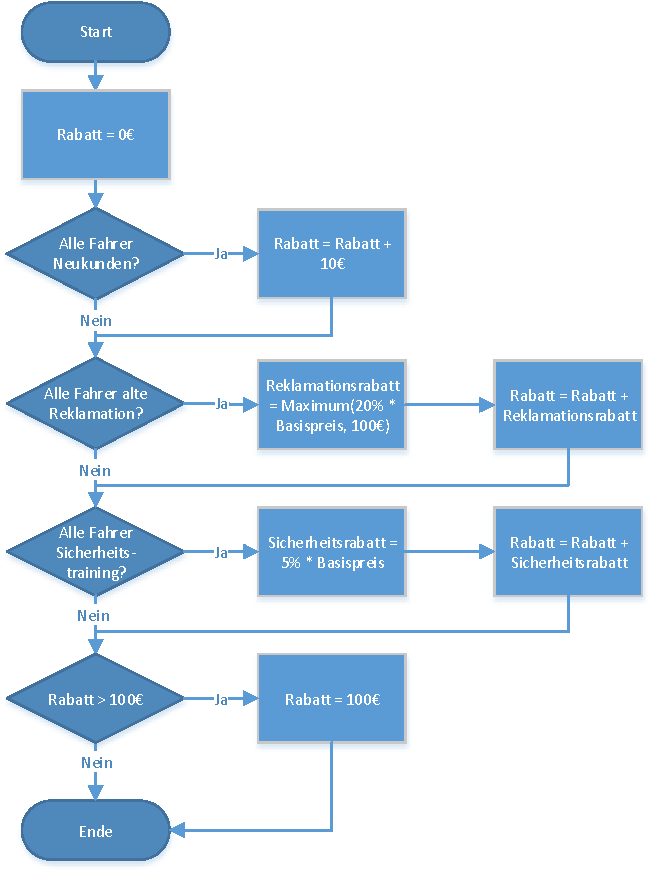
\includegraphics[width=0.8\linewidth]{Bilder/Rabatt_berechnen}
	\caption{Rabatt berechnen}
	\label{fig:Rabatt_berechnen}
\end{figure}

\section{Regeln und Prozesse}

Aus den Aussagen und dem Flussdiagramm ergibt sich folgender grober Prozessablauf:
\begin{enumerate}
	\item Fahranfängerprüfung
	\item Ggf. Genehmigung der Fahrzeugklasse durch den Filialleiter
	\item Verfügbarkeitsprüfung
	\item Ggf. Genehmigung des Upgrades durch den Filialleiter
	\item Preisberechnung
\end{enumerate}

Die Genehmigungen sind manuelle Prozesse, die durch den Filialleiter durchgeführt werden müssen.
Die Fahranfängerprüfung, die Verfügbarkeitsprüfung sowie die Preisberechnung lassen sich über
Geschäftsregeln abbilden. 
Im Folgenden beschreiben wir die Regeln, die wir aus den Aussagen der Aufgabenstellung
extrahiert haben.

\subsection{Fahranfängerprüfung}

Regel: Definition eines Fahranfängers \\
Kategorie: Definitionsregel

\begin{lstlisting}
rule "Is driving novice" ruleflow-group "novice-check"
	when
		there is a request
		there is a customer with that request
		- age is less than 21 or has driving license for less than 2	
	then
		the customer is a driving novice	
end
\end{lstlisting}

Regel: Zuschlag für Fahranfänger \\
Kategorie: Prozessregel

\begin{lstlisting}
rule "Extra charge if at least one customer is a novice" ruleflow-group "novice-check"
	when
		there is a request
		there exists a customer who is driving novice
	then
		treat the request as novice
		set extra charge to 10%	
end
\end{lstlisting}

Regel: Genehmigung für höhere Klassen bei Fahranfängern \\
Kategorie: Prozessregel

\begin{lstlisting}
rule "Permission for higher classes required" ruleflow-group "novice-check"
	when
		there is a request
		- car class is not in ("Small", "Compact")
		there exists a customer who is driving novice
	then
		ask the boss for permission
end
\end{lstlisting}

\subsection{Verfügbarkeitsprüfung}

Regel: Downgrade aus Oberklasse, wenn nicht verfügbar \\
Kategorie: Prozessregel

\begin{lstlisting}
rule "Downgrade for upper class if not available" ruleflow-group "availibility-check"
	when
		there is a request
		- car class is "Upper"
		- car is not available
	then
		set car class to "Middle"
		set extra deduction to 10%
		update the request
end
\end{lstlisting}

Regel: Definition eines Upgrades für die Fahrzeugklasse \\
Kategorie: Definitionsregel

Es gibt eine Reihe von Regeln, die definieren welche Fahrzeugklassen ein Upgrade
für die angefragte Klasse darstellen. Folgende Regel ist ein Beispiel von
Klein- nach Kompaktwagen.

\begin{lstlisting}
rule "Upgrade from Small to Compact" ruleflow-group "availibility-check"
	when
		there is a request
		- car class is "Small"
		- "Compact" car is available
		there exists no upgrade
	then
		upgrade to "Compact" is possible	
end
\end{lstlisting}

Regel: Upgrade auf nächsthöhere Klasse, wenn nicht verfügbar \\
Kategorie: Prozessregel

\begin{lstlisting}
rule "If updgrade possible it requires permission" ruleflow-group "availibility-check"
	when
		there is a request
		- car is not available
		there is a possible upgrade
	then
		upgrade the car class
		mark the car for that request as available
end
\end{lstlisting}

\subsection{Preisberechnung}

Regel: Definition des Tagespreises \\
Kategorie: Definitionsregel

Es gibt eine Reihe von Regeln, die den Tagespreis für jede Fahrzeugklasse festlegen.
Folgende Regel ist ein Beispiel für Kleinwagen.

\begin{lstlisting}
rule "Daily price: Small class car" ruleflow-group "price-calculation"
	when
		there is a request
		- car class is "Small"
		there is a rental day from that request
	then
		set the daily price to 40.00
end
\end{lstlisting}

Regel: Wochenenden und Feiertage haben reduzierten Tagespreis \\
Kategorie: Ableitungsregel

\begin{lstlisting}
rule "Daily price: Weekend discount" ruleflow-group "price-calculation"
	when
		there is a request
		there is a rental day from that request
		- is weekend or holiday
	then
		the daily price is discounted by 25%
end
\end{lstlisting}

Regel: Jeder siebte Tag ist kostenlos \\
Kategorie: Ableitungsregel

\begin{lstlisting}
rule "Daily price: Free seventh day" ruleflow-group "price-calculation"
	when
		there is a request
		there is a rental day from that request
		- day index is in (7, 14, 21, 28)
	then
		set the daily price to 0.00
end
\end{lstlisting}

Regel: Basispreis ist die Summe der Tagespreise \\
Kategorie: Ableitungsregel

\begin{lstlisting}
rule "Base price is the sum of daily prices" ruleflow-group "price-calculation"
	when
		there is a request
		there is a rental day from that request
	then
		add the daily price to the base price
end
\end{lstlisting}

Regel: Neukundenrabatt \\
Kategorie: Ableitungsregel

\begin{lstlisting}
rule "Discount: All customers are new customers" ruleflow-group "price-calculation"
	when
		there is a request
		every customer from that request is a new customer
	then
		add 10.00 to the discount
end
\end{lstlisting}

Regel: Reklamationsrabatt \\
Kategorie: Ableitungsregel

\begin{lstlisting}
rule "Discount: All customers have an old reclamation" ruleflow-group "price-calculation"
	when
		there is a request
		every customer from that request had a valid reclamation
	then
		discount the base price by 20%
end
\end{lstlisting}

Regel: Rabatt für Sicherheitstraining \\
Kategorie: Ableitungsregel

\begin{lstlisting}
rule "Discount: All customers have participated in security training" ruleflow-group "price-calculation"
	when
		there is a request
		every customer from that request had a security training
	then
		discount the base price by 5%;
end
\end{lstlisting}

Regel: Maximaler Rabatt \\
Kategorie: Einschränkungsregel

\begin{lstlisting}
rule "Discount is limited to 100 Euro" ruleflow-group "price-calculation"
	when
		there is a request
		- discount is greater than 100.00
	then
		set the discount to 100.00
end
\end{lstlisting}

Regel: Endpreis berechnen \\
Kategorie: Ableitungsregel

\begin{lstlisting}
rule "Final Price: Calculation" ruleflow-group "price-calculation"
	when
		there is a request
	then
		set the final price to the base price
		subtract the discount from the final price
end
\end{lstlisting}

Regel: Automatikgebühr abziehen \\
Kategorie: Ableitungsregel

\begin{lstlisting}
rule "Final Price: Automatic fee" ruleflow-group "price-calculation"
	when
		there is a request
		- for an automatic car
	then
		add a 5% fee of the base price to the final price
end
\end{lstlisting}

Regel: Gesamtpreis berechnen \\
Kategorie: Ableitungsregel

\begin{lstlisting}
rule "Total Price" ruleflow-group "price-calculation"
	when
		there is a request
	then
		set percent to 100% plus extra charge minus extra deduction
		set the total price to percent% of the final price
end
\end{lstlisting}

\section{Anwendungssituation}
\label{sec:Anwendungssituation}

Wir analysieren die Situation am 21. März 2016 in der Autovermietungsstation.
Dazu beschreiben wir zunächst die Ausgangssituation und dann die einzelnen Kundenanfragen.

\subsection{Ausgangssituation}

Am 21. März 2016 stehen zu jeder Fahrzeugklasse zwei Fahrzeuge zur Verfügung:

\begin{tabular}{|c|c|c|c|}
	\hline \textbf{Kleinklasse} & \textbf{Kompaktklasse} & \textbf{Mittelklasse} & \textbf{Oberklasse}  \\ 
	\hline 2 & 2 & 2 & 2 \\ 
	\hline 
\end{tabular} 

Relevante Feiertage:
\begin{itemize}
	\item Fr 25.03.2016: Karfreitag
	\item Mo 28.03.2016: Ostermontag
	\item So 01.05.2016: 1. Mai / Tag der Arbeit
\end{itemize}

Vorgehen:
\begin{itemize}
	\item Wir runden mathematisch, weil das einfacher zu implementieren ist.
	\item Nicht spezifizierte Anfrageparameter nehmen einen Standardwert an (Nein, bzw. 0).
	\item Bei nicht angegebenem Alter ist der Kunde älter als 21 Jahre.
	\item Der Filialleiter genehmigt alle Anfragen.
	\item Wenn die Anfrage abgelehnt wird, weil keine Wagen der angefragten Klasse vorhanden sind,
		wird als Alternative dieselbe Anfrage mit vorhandener Klasse betrachtet.
\end{itemize}

\subsection{Kunde A}

Kundendaten:\\
\begin{tabular}{|c|c|c|c|c|}
	\hline \textbf{Alter} & \textbf{Führerschein} & \textbf{Neukunde} & \textbf{Reklamation} & \textbf{Sicherheitstraining} \\ 
	\hline 42 & 20 & Nein & Nein & Ja \\ 
	\hline 
\end{tabular} 
\\\\
Anfrage:\\
\begin{tabular}{|c|c|c|}
	\hline \textbf{Klasse} & \textbf{Dauer in Tagen} & \textbf{Automatik} \\ 
	\hline Mittel & 5 & Nein \\ 
	\hline 
\end{tabular}

\vspace{12pt}
Preisberechnung:
\begin{itemize}
	\item Zeitraum: 4 Wochentage, 0 Wochenende, 1 Feiertag
	\item Fahranfängerprüfung: Bestanden, Zuschlag: 0\%
	\item Verfügbarkeitsprüfung: Bestanden, Nachlass: 0\%
	\item Tagespreis: 70€/Wochentag, 52,50€/Feiertag
	\item Basispreis = 70€ * 4 + 52,50€ * 1 = 332,50€
	\item Rabatt = 5\% * Basispreis = 16,63€
	\item Endpreis = 315,87€
	\item Gesamtpreis = Endpreis = 315,87€
\end{itemize}

Zustand nach Vermietung:\\
\begin{tabular}{|c|c|c|c|}
	\hline \textbf{Kleinklasse} & \textbf{Kompaktklasse} & \textbf{Mittelklasse} & \textbf{Oberklasse}  \\ 
	\hline 2 & 2 & 1 & 2 \\ 
	\hline 
\end{tabular} 

\subsection{Kunde B}

Kundendaten:\\
\begin{tabular}{|c|c|c|c|c|}
	\hline \textbf{Alter} & \textbf{Führerschein} & \textbf{Neukunde} & \textbf{Reklamation} & \textbf{Sicherheitstraining} \\ 
	\hline 20 & 3 & Ja & Nein & Nein \\ 
	\hline 
\end{tabular} 
\\\\
Anfrage:\\
\begin{tabular}{|c|c|c|}
	\hline \textbf{Klasse} & \textbf{Dauer in Tagen} & \textbf{Automatik} \\ 
	\hline Mittel & 1 & Nein \\ 
	\hline 
\end{tabular}

Preisberechnung:
\begin{itemize}
	\item Zeitraum: 1 Wochentag, 0 Wochenende oder Feiertage
	\item Fahranfängerprüfung: Genehmigung, Bestanden, Zuschlag: 10\%
	\item Verfügbarkeitsprüfung: Bestanden, Nachlass: 0\%
	\item Tagespreis: 70€/Wochentag, 52,50€/Feiertag
	\item Basispreis = 70€ * 1 + 52,50€ * 0 = 70,00€
	\item Rabatt = 10,00€
	\item Endpreis = 60,00€
	\item Gesamtpreis = 110\% * Endpreis = 66,00€
\end{itemize}

Zustand nach Vermietung:\\
\begin{tabular}{|c|c|c|c|}
	\hline \textbf{Kleinklasse} & \textbf{Kompaktklasse} & \textbf{Mittelklasse} & \textbf{Oberklasse}  \\ 
	\hline 2 & 2 & 0 & 2 \\ 
	\hline 
\end{tabular} 

\subsection{Kunde C}

Kundendaten:\\
\begin{tabular}{|c|c|c|c|c|}
	\hline \textbf{Alter} & \textbf{Führerschein} & \textbf{Neukunde} & \textbf{Reklamation} & \textbf{Sicherheitstraining} \\ 
	\hline 30 & 12 & Nein & Nein & Nein \\ 
	\hline 
\end{tabular} 
\\\\
Anfrage:\\
\begin{tabular}{|c|c|c|}
	\hline \textbf{Klasse} & \textbf{Dauer in Tagen} & \textbf{Automatik} \\ 
	\hline Mittel & 7 & Nein \\ 
	\hline 
\end{tabular}

Zwischenergebnis:
\begin{itemize}
	\item Zeitraum: 4 Wochentag, 2 Wochenende oder Feiertage, 1 Gratistag
	\item Fahranfängerprüfung: Bestanden, Zuschlag: 0\%
	\item Verfügbarkeitsprüfung: Genehmigung, Bestanden, Upgrade auf höhere Klasse, Nachlass: 0\%
	\item Tagespreis: 70€/Wochentag, 52,50€/Feiertag
	\item Basispreis = 70€ * 4 + 52,50€ * 2 + 0€ * 1 = 385,00€
	\item Rabatt = 0,00€
	\item Endpreis = 385,00€
	\item Gesamtpreis = 100\% * Endpreis = 385,00€
\end{itemize}

Zustand nach Vermietung:\\
\begin{tabular}{|c|c|c|c|}
	\hline \textbf{Kleinklasse} & \textbf{Kompaktklasse} & \textbf{Mittelklasse} & \textbf{Oberklasse}  \\ 
	\hline 2 & 2 & 0 & 1 \\ 
	\hline 
\end{tabular} 

\subsection{Kunde D}

Kundendaten:\\
\begin{tabular}{|c|c|c|c|c|}
	\hline \textbf{Alter} & \textbf{Führerschein} & \textbf{Neukunde} & \textbf{Reklamation} & \textbf{Sicherheitstraining} \\ 
	\hline 35 & 10 & Ja & Nein & Nein \\ 
	\hline 
\end{tabular} 
\\\\
Anfrage:\\
\begin{tabular}{|c|c|c|}
	\hline \textbf{Klasse} & \textbf{Dauer in Tagen} & \textbf{Automatik} \\ 
	\hline Mittel & 1 & Nein \\ 
	\hline 
\end{tabular}

Preisberechnung:
\begin{itemize}
	\item Zeitraum: 1 Wochentag, 0 Wochenende oder Feiertage
	\item Fahranfängerprüfung: Bestanden, Zuschlag: 0\%
	\item Verfügbarkeitsprüfung: Genehmigung, Bestanden, Upgrade auf höhere Klasse, Nachlass: 0\%
	\item Tagespreis: 70€/Wochentag, 52,50€/Feiertag
	\item Basispreis = 70€ * 1 + 52,50€ * 0 = 70,00€
	\item Rabatt = 10,00€
	\item Endpreis = 60,00€
	\item Gesamtpreis = 100\% * Endpreis = 60,00€
\end{itemize}

Zustand nach Vermietung:\\
\begin{tabular}{|c|c|c|c|}
	\hline \textbf{Kleinklasse} & \textbf{Kompaktklasse} & \textbf{Mittelklasse} & \textbf{Oberklasse}  \\ 
	\hline 2 & 2 & 0 & 0 \\ 
	\hline 
\end{tabular}

\subsection{Kunde E (abgelehnt)}

Kundendaten:\\
\begin{tabular}{|c|c|c|c|c|}
	\hline \textbf{Alter} & \textbf{Führerschein} & \textbf{Neukunde} & \textbf{Reklamation} & \textbf{Sicherheitstraining} \\ 
	\hline 46 & 20 & Ja & Nein & Nein \\ 
	\hline 
\end{tabular} 
\\\\
Anfrage:\\
\begin{tabular}{|c|c|c|}
	\hline \textbf{Klasse} & \textbf{Dauer in Tagen} & \textbf{Automatik} \\ 
	\hline Ober & 6 & Nein \\ 
	\hline 
\end{tabular}

Preisberechnung:
\begin{itemize}
	\item Zeitraum: 4 Wochentag, 2 Wochenende oder Feiertage
	\item Fahranfängerprüfung: Bestanden, Zuschlag: 0\%
	\item Verfügbarkeitsprüfung: Genehmigung, Abgelehnt, Nachlass: 10\%, Klasse = Mittel
	
	% Es gibt noch eine Oberklasse:
	%\item Tagespreis: 90€/Wochentag, 67,50€/Feiertag
	%\item Basispreis = $90€ * 4 + 67,50€ * 2 = 495,00€$
%	\item Rabatt = 10,00€
%	\item Endpreis = 485,00€
%	\item Gesamtpreis = 100\% * Endpreis = 485,00€
	
	% Es gibt keine Oberklasse aber eine Mittelklasse
%	\item Tagespreis: 70€/Wochentag, 52,50€/Feiertag
%	\item Basispreis = $70€ * 4 + 52,50€ * 2 = 385,00€$
%	\item Rabatt = 10,00€
%	\item Endpreis = 375,00€
%	\item Gesamtpreis = 90\% * Endpreis = 337,50€
\end{itemize}

Abgelehnt: Keine Änderung
Zustand nach Vermietung:\\
\begin{tabular}{|c|c|c|c|}
	\hline \textbf{Kleinklasse} & \textbf{Kompaktklasse} & \textbf{Mittelklasse} & \textbf{Oberklasse}  \\ 
	\hline 2 & 2 & 0 & 0 \\ 
	\hline 
\end{tabular}

\subsection{Kunde F (abgelehnt)}

Kundendaten:\\
\begin{tabular}{|c|c|c|c|c|}
	\hline \textbf{Alter} & \textbf{Führerschein} & \textbf{Neukunde} & \textbf{Reklamation} & \textbf{Sicherheitstraining} \\ 
	\hline 32 & 10 & Nein & Nein & Ja \\ 
	\hline 
\end{tabular} 
\\\\
Anfrage:\\
\begin{tabular}{|c|c|c|}
	\hline \textbf{Klasse} & \textbf{Dauer in Tagen} & \textbf{Automatik} \\ 
	\hline Ober & 4 & Nein \\ 
	\hline 
\end{tabular}

Zwischenergebnis:
\begin{itemize}
	\item Zeitraum: 4 Wochentag, 0 Wochenende oder Feiertage
	\item Fahranfängerprüfung: Bestanden, Zuschlag: 0\%
	\item Verfügbarkeitsprüfung: Genehmigung, Abgelehnt, Nachlass: 0\%
%	\item Tagespreis: 90€/Wochentag, 67,50€/Feiertag
%	\item Basispreis = $90€ * 4 + 67,50€ * 0 = 360,00€$
%	\item Rabatt = 20\% * 360€ + 5\% * 360€ = 72€ + 18€ = 90€
%	\item Endpreis = 270,00€
%	\item Gesamtpreis = 100\% * Endpreis = 270,00€
	
	% Siehe E
\end{itemize}

Abgelehnt: Keine Änderung
Zustand nach Vermietung:\\
\begin{tabular}{|c|c|c|c|}
	\hline \textbf{Kleinklasse} & \textbf{Kompaktklasse} & \textbf{Mittelklasse} & \textbf{Oberklasse}  \\ 
	\hline 2 & 2 & 0 & 0 \\ 
	\hline 
\end{tabular}

\subsection{Kunde G}

Kundendaten:\\
\begin{tabular}{|c|c|c|c|c|}
	\hline \textbf{Alter} & \textbf{Führerschein} & \textbf{Neukunde} & \textbf{Reklamation} & \textbf{Sicherheitstraining} \\ 
	\hline 30 & 6 & Nein & Nein & Ja \\ 
	\hline 25 & 1 & Nein & Nein & Nein \\ 
	\hline 
\end{tabular} 
\\\\
Anfrage:\\
\begin{tabular}{|c|c|c|}
	\hline \textbf{Klasse} & \textbf{Dauer in Tagen} & \textbf{Automatik} \\ 
	\hline Kompakt & 1 & Nein \\ 
	\hline 
\end{tabular}

Zwischenergebnis:
\begin{itemize}
	\item Zeitraum: 1 Wochentag, 0 Wochenende oder Feiertage
	\item Fahranfängerprüfung: Bestanden, Zuschlag: 10\%
	\item Verfügbarkeitsprüfung: Bestanden, Nachlass: 0\%
	\item Tagespreis: 50€/Wochentag, 37,50€/Feiertag
	\item Basispreis = 50€ * 1 + 37,50€ * 0 = 50,00€
	\item Rabatt = 0€
	\item Endpreis = 50,00€
	\item Gesamtpreis = 110\% * Endpreis = 55,00€
\end{itemize}

Zustand nach Vermietung:\\
\begin{tabular}{|c|c|c|c|}
	\hline \textbf{Kleinklasse} & \textbf{Kompaktklasse} & \textbf{Mittelklasse} & \textbf{Oberklasse}  \\ 
	\hline 2 & 2 & 0 & 0 \\ 
	\hline 
\end{tabular}

\subsection{Kunde E (angenommen)}

Wir nehmen an, es gäbe ausreichend Wagen jeder Klasse:

\begin{tabular}{|c|c|c|c|}
	\hline \textbf{Kleinklasse} & \textbf{Kompaktklasse} & \textbf{Mittelklasse} & \textbf{Oberklasse}  \\ 
	\hline 2 & 2 & 2 & 2 \\ 
	\hline 
\end{tabular}

Kundendaten:\\
\begin{tabular}{|c|c|c|c|c|}
	\hline \textbf{Alter} & \textbf{Führerschein} & \textbf{Neukunde} & \textbf{Reklamation} & \textbf{Sicherheitstraining} \\ 
	\hline 46 & 20 & Ja & Nein & Nein \\ 
	\hline 
\end{tabular} 
\\\\
Anfrage:\\
\begin{tabular}{|c|c|c|}
	\hline \textbf{Klasse} & \textbf{Dauer in Tagen} & \textbf{Automatik} \\ 
	\hline Ober & 6 & Nein \\ 
	\hline 
\end{tabular}

Preisberechnung:
\begin{itemize}
	\item Zeitraum: 4 Wochentag, 2 Wochenende oder Feiertage
	\item Fahranfängerprüfung: Bestanden, Zuschlag: 0\%
	\item Verfügbarkeitsprüfung: Bestanden, Nachlass: 0\%
	
	% Es gibt noch eine Oberklasse:
	\item Tagespreis: 90€/Wochentag, 67,50€/Feiertag
	\item Basispreis = $90€ * 4 + 67,50€ * 2 = 495,00€$
	\item Rabatt = 10,00€
	\item Endpreis = 485,00€
	\item Gesamtpreis = 100\% * Endpreis = 485,00€
	
	% Es gibt keine Oberklasse aber eine Mittelklasse
	%	\item Tagespreis: 70€/Wochentag, 52,50€/Feiertag
	%	\item Basispreis = $70€ * 4 + 52,50€ * 2 = 385,00€$
	%	\item Rabatt = 10,00€
	%	\item Endpreis = 375,00€
	%	\item Gesamtpreis = 90\% * Endpreis = 337,50€
\end{itemize}

Zustand nach Vermietung:\\
\begin{tabular}{|c|c|c|c|}
	\hline \textbf{Kleinklasse} & \textbf{Kompaktklasse} & \textbf{Mittelklasse} & \textbf{Oberklasse}  \\ 
	\hline 2 & 2 & 2 & 1 \\ 
	\hline 
\end{tabular}

\subsection{Kunde F (angenommen)}

Wir nehmen an, es gäbe ausreichend Wagen jeder Klasse:

\begin{tabular}{|c|c|c|c|}
	\hline \textbf{Kleinklasse} & \textbf{Kompaktklasse} & \textbf{Mittelklasse} & \textbf{Oberklasse}  \\ 
	\hline 2 & 2 & 2 & 2 \\ 
	\hline 
\end{tabular}

Kundendaten:\\
\begin{tabular}{|c|c|c|c|c|}
	\hline \textbf{Alter} & \textbf{Führerschein} & \textbf{Neukunde} & \textbf{Reklamation} & \textbf{Sicherheitstraining} \\ 
	\hline 32 & 10 & Nein & Nein & Ja \\ 
	\hline 
\end{tabular} 
\\\\
Anfrage:\\
\begin{tabular}{|c|c|c|}
	\hline \textbf{Klasse} & \textbf{Dauer in Tagen} & \textbf{Automatik} \\ 
	\hline Ober & 4 & Nein \\ 
	\hline 
\end{tabular}

Zwischenergebnis:
\begin{itemize}
	\item Zeitraum: 4 Wochentag, 0 Wochenende oder Feiertage
	\item Fahranfängerprüfung: Bestanden, Zuschlag: 0\%
	\item Verfügbarkeitsprüfung: Bestanden, Nachlass: 0\%
	\item Tagespreis: 90€/Wochentag, 67,50€/Feiertag
	\item Basispreis = 90€ * 4 + 67,50€ * 0 = 360,00€
	\item Rabatt = 20\% * 360€ + 5\% * 360€ = 72€ + 18€ = 90€
	\item Endpreis = 270,00€
	\item Gesamtpreis = 100\% * Endpreis = 270,00€
	
	% Siehe E
\end{itemize}

Abgelehnt: Keine Änderung
Zustand nach Vermietung:\\
\begin{tabular}{|c|c|c|c|}
	\hline \textbf{Kleinklasse} & \textbf{Kompaktklasse} & \textbf{Mittelklasse} & \textbf{Oberklasse}  \\ 
	\hline 2 & 2 & 2 & 1 \\ 
	\hline 
\end{tabular}

\section{Prototyp}

Die Umsetzung des Prototypen haben wir in vier Schritte eingeteilt:
\begin{enumerate}
	\item Festlegung des Datenmodells
	\item Schreiben von Unit-Tests
	\item Implementierung der Regeln
	\item Transformation der Regeln in eine DSL 
\end{enumerate}

\subsection{Datenmodell}

Die zu modellierenden Daten umfassen Kunden- und Anfragedaten. Diese beiden Datensätze
werden als Java-Klassen modelliert (Customer und RentalRequest). Zusätzlich werden die
Informationen über die zur Verfügung stehenden Autos in die Klasse Garage gespeichert.
Die einzelnen Miettage werden als RentalDay modelliert. Das Klassendiagramm in
Abbildung \ref{fig:Class_All} zeigt alle Klassen.

\begin{figure}[tbh]
\centering
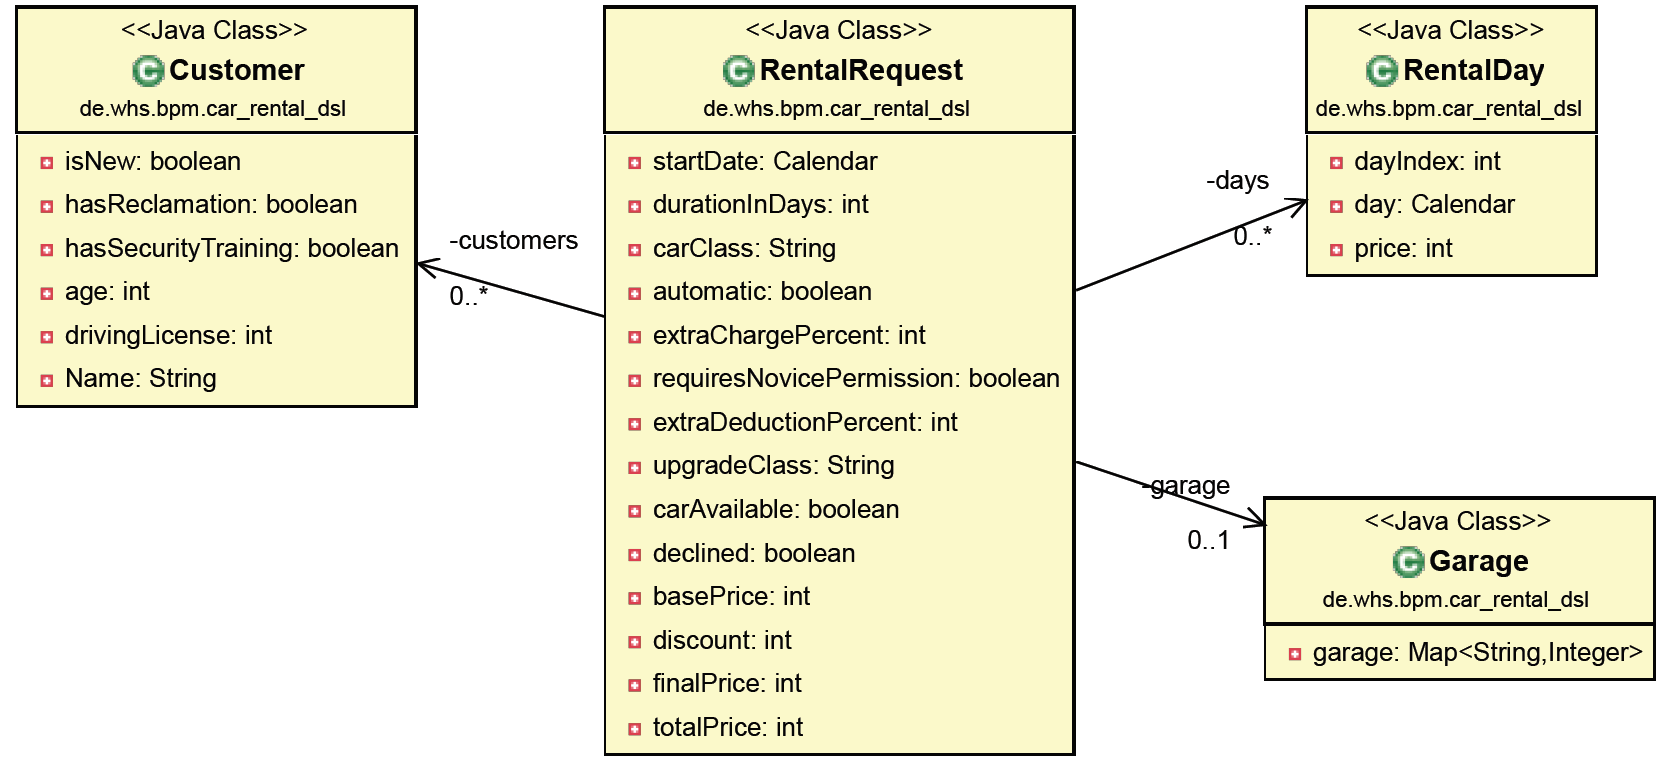
\includegraphics[width=1.0\linewidth]{Bilder/Class_All}
\caption{Klassendiagramm}
\label{fig:Class_All}
\end{figure}

Die Klasse RentalRequest dient sowohl der Eingabe als auch der Ausgabe von Daten.
Das heißt, dass Regeln und Prozesse ggf. schreibend auf die aktuelle Instanz zugreifen.

\subsection{Unit-Tests: Anwendungssituation}

Nachdem wir das Datenmodell festgelegt haben, konnten wir Unit-Tests für die 
Anwendungssituationen aus der Aufgabenstellung schreiben. Dabei ist uns aufgefallen,
dass bei sequentieller Abarbeitung der Kunden A bis G die Wagen der Mittel- und
Oberklasse schnell ausgehen. Dies führt dazu dass die Anfragen der Kunden E und F
direkt abgelehnt werden. Für die Unit-Tests haben wir zusätzlich die Fälle betrachtet,
wenn es genügend Wagen in der angeforderten Klasse gibt.

Die erwarteten Preise in den einzelnen Anwendungssituationen haben wir manuell
mithilfe des initial erstellten Flussdiagramms ermittelt. Die Ergebnisse dieser
manuellen Auswertung befinden sich in Anhang \ref{sec:Anwendungssituation}.

In der Java-Klasse SituationTest werden die vorgegebenen Situationen getestet.
Zusätzlich haben wir in der Klasse ExtraTest versucht, bisher noch nicht
getestete Szenarien abzubilden. Dazu zählen z.~B. die Automatikgebühr und verschiedene
Genehmigungszenarien.

\subsection{Definition des Geschäftsprozesses}

Die Autovermietung ist ein Geschäftsprozess, in dem unterschiedliche Regelgruppen aktiviert
werden müssen. Außerdem ist ja nach Anfrage eine menschliche Interaktion durch den
Filialleiter in Form einer Genehmigung erforderlich. Dies haben wir mittels
jBPM als Prozess definiert.

Die Integration der Geschäftsregeln haben wir durch die Zuordnung zu Ruleflow-Groups
in der Regeldatei und das Einbinden von Business-Rule-Tasks in den Prozess.
Um die Genehmigung durch den Filialleiter zu ermöglichen haben wir User- bzw.
Human-Tasks eingebunden.

Der gesamte Prozess wird in Abbildung \ref{fig:Process_BPMN} dargestellt.

\begin{figure}[tbh]
\centering
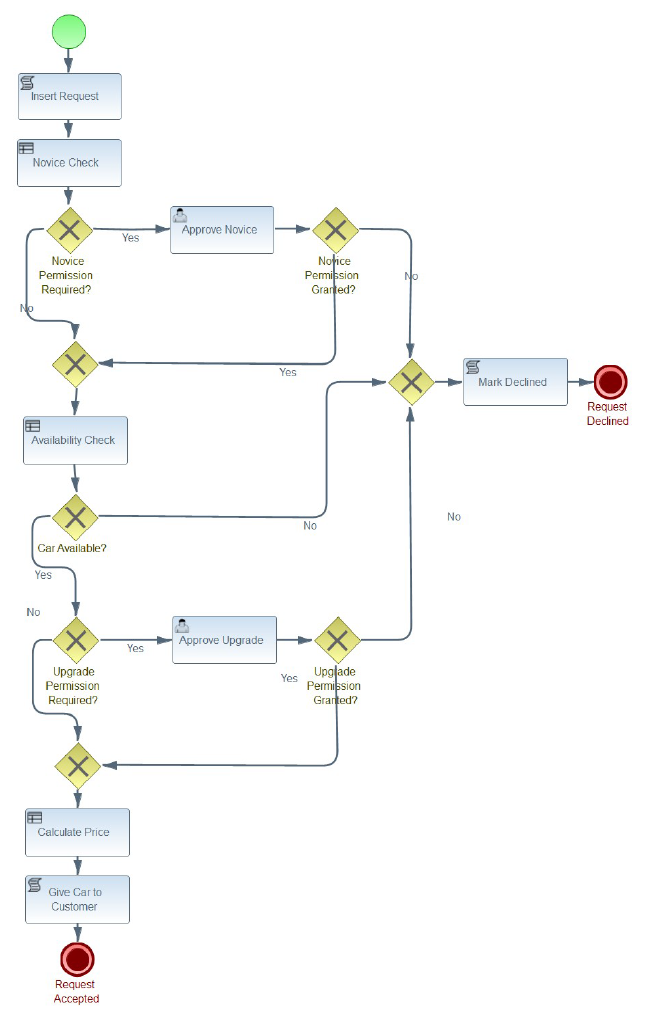
\includegraphics[width=0.8\linewidth]{Bilder/Process_BPMN}
\caption{Geschäftsprozess in jBPM}
\label{fig:Process_BPMN}
\end{figure}

\subsection{Umsetzung mittels einfacher Regeldatei}

Um mögliche Fehlerquellen zu vermeiden, haben wir die Geschäftsregeln 

\subsection{Nutzung einer DSL}

\subsection{Unit-Tests}
Tests für die Anwendungssituation.

\subsection{Oberfläche}
Zur einfachen Eingabe von Testfällen habe wir eine Java SWING GUI Programmiert. Diese besteht aus einer Haupt-Eingabemaske \ref{fig:Autovermietung} über die ein Mietgesuch eingegeben werden kann, einem Fahrer Verwaltungs-Dialog \ref{fig:kunde} und einem Garagen Konfigurations-Dialog \ref{fig:Garage}. Der Dialog zum Verwalten der Fahrer ermöglicht eingaben über den Name des Fahrers, das Alter des Fahrers, wie lange der Fahrer schon einen Führerschein besitzt, ob er ein Neukunde ist, eine Reklamation vorweisen kann und ob er ein Sicherheitstraining absolviert hat. Über den Garagen Konfigurations-Dialog kann die Anzahl der zu Verfügung stehenden Fahrzeuge in den einzelnen Fahrzeugklassen eingestellt werden. In der Haupt-Eingabemaske kann der Garagendialog aufgerufen werden und es können Fahrer über den Fahrerdialog hinzugefügt und verwaltet werden. Alle Fahrer einer Mietanfrage werden im Hauptfenster Angezeigt. Das Hauptfenster bietet die Möglichkeit zum einstellen des Mietstartdatums, der Mietdauer, der Fahrzeugklasse des Mietwagens und ob der Mietwagen eine Automatikschaltung haben soll. 

Nachdem alle Eingaben gemacht wurden kann eine Mietanfrage an das System gesendet werden. Abhängig von den Eingabewerten muss ein Fahranfänger \ref{fig:Fahränfanger} oder ein Fahrzeugupgrade \ref{fig:Upgrade} genehmigt werden. Wird eine Genehmigung nicht erteilt oder steht kein Fahrzeug mehr zur Verfügung wird die Anfrage abgelehnt \ref{fig:ergebnisabgelehnt}. Sollte die Anfrage berechnet werden, wird in einem abschließendem Dialog die Fahrzeugklasse und die zu zahlenden Kosten angezeigt \ref{fig:ergebnis}.


\begin{figure}
\centering
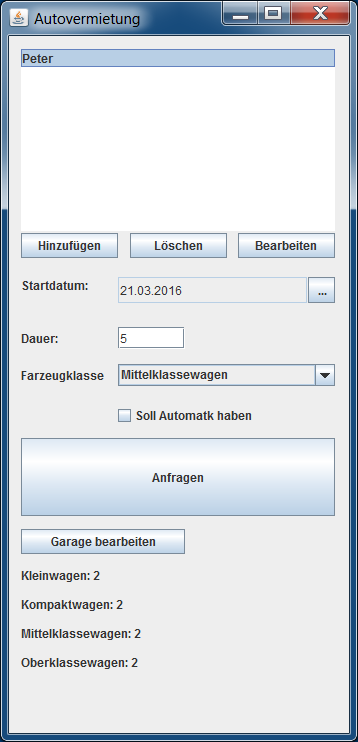
\includegraphics[width=0.7\linewidth]{Bilder/Screenshots/Autovermietung}
\caption{Haupt-Eingabemaske }
\label{fig:Autovermietung}
\end{figure}


\begin{figure}
\centering
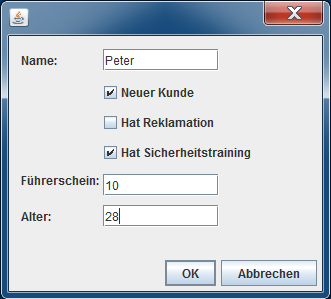
\includegraphics[width=0.7\linewidth]{Bilder/Screenshots/kunde}
\caption{Kundendialog}
\label{fig:kunde}
\end{figure}

\begin{figure}
	\centering
	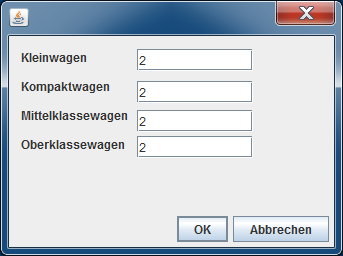
\includegraphics[width=0.7\linewidth]{Bilder/Screenshots/Garage}
	\caption{Garagendialog}
	\label{fig:Garage}
\end{figure}

\begin{figure}
	\centering
	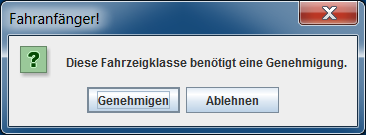
\includegraphics[width=0.7\linewidth]{Bilder/Screenshots/Fahranfanger}
	\caption{Fahranfänger genehmigen}
	\label{fig:Fahränfanger}
\end{figure}

\begin{figure}
	\centering
	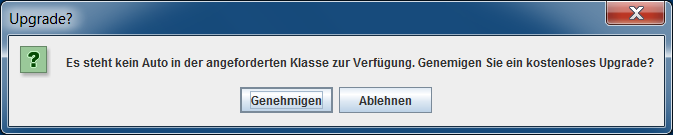
\includegraphics[width=0.7\linewidth]{Bilder/Screenshots/Upgrade}
	\caption{Fahrzeugklassen Upgrade genehmigen}
	\label{fig:Upgrade}
\end{figure}

\begin{figure}
	\centering
	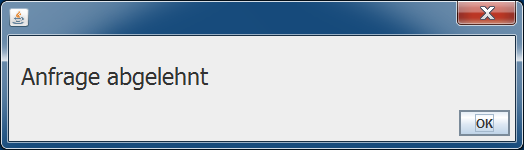
\includegraphics[width=0.7\linewidth]{Bilder/Screenshots/ergebnis-abgelehnt}
	\caption{Anfrage abgelehnt}
	\label{fig:ergebnisabgelehnt}
\end{figure}

\begin{figure}
	\centering
	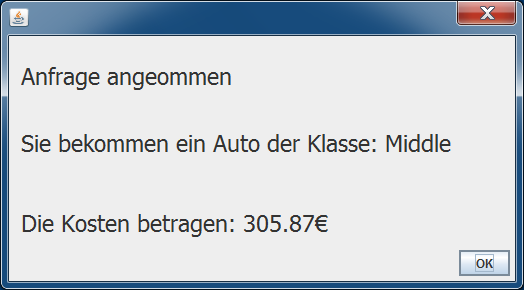
\includegraphics[width=0.7\linewidth]{Bilder/Screenshots/ergebnis}
	\caption{Ergebnis einer genehmigten Anfrage}
	\label{fig:ergebnis}
\end{figure}

\section{Fazit}

Vorgehen:
- Ausarbeitung von Regeln aus den Aussagen
- Zunächst in die normale Regelsprache um zu sehen das es funktioniert
- Übersetzung in DSL: Fehlerquellen vermeiden

DSL: Weg von der abstrakten Grammatik
- Eine Fachperson kann die Regeln lesen: Bestätigen, Fehler finden
- Halber Entwickler: Kann die Regeln ggf. anpassen
- Feste Struktur: Keine beliebigen Sätze ==> Programmierwissen

Framework:
- Interaktion zwischen Prozessen und Regeln (Drools + jBPM): Relativ einfach
- Unit-Tests schreiben war schnell möglich
- Integration in die GUI: schnell und hat funktioniert

%\appendix
%\include{Inhalt/Anhang}

%\newpage
%\printbibliography

\end{document}